\documentclass[a4paper,14pt]{extreport} % формат документа

\usepackage{amsmath}
\usepackage{cmap} % поиск в ПДФ
\usepackage[T2A]{fontenc} % кодировка
\usepackage[utf8]{inputenc} % кодировка исходного текста
\usepackage[english,russian]{babel} % локализация и переносы
\usepackage[left = 2cm, right = 1cm, top = 2cm, bottom = 2 cm]{geometry} % поля
\usepackage{listings}
\usepackage{graphicx} % для вставки рисунков
\usepackage{amsmath}
\usepackage{float}
\usepackage{longtable}
\usepackage{multirow}
\usepackage{pdfpages}
\graphicspath{{pictures/}}
\DeclareGraphicsExtensions{.pdf,.png,.jpg}
\newcommand{\anonsection}[1]{\section*{#1}\addcontentsline{toc}{section}{#1}}

	\lstset{ %
	language=C,                % Язык программирования 
	numbers=left,                   % С какой стороны нумеровать          
	frame=single,                    % Добавить рамку
	basicstyle=\small,
	keywordstyle=\color{blue}\ttfamily,
	    stringstyle=\color{red}\ttfamily,
	    commentstyle=\color{blue!20!black!30!green}\ttfamily,
	    morecomment=[l][\color{magenta}]{\#},
	    columns=fullflexible,
	    keepspaces=true,
    escapebegin=\begin{russian}\commentfont,
    escapeend=\end{russian},
    literate={Ö}{{\"O}}1
    {Ä}{{\"A}}1
    {Ü}{{\"U}}1
    {ß}{{\ss}}1
    {ü}{{\"u}}1
    {ä}{{\"a}}1
    {ö}{{\"o}}1
    {~}{{\textasciitilde}}1
    {а}{{\selectfont\char224}}1
    {б}{{\selectfont\char225}}1
    {в}{{\selectfont\char226}}1
    {г}{{\selectfont\char227}}1
    {д}{{\selectfont\char228}}1
    {е}{{\selectfont\char229}}1
    {ё}{{\"e}}1
    {ж}{{\selectfont\char230}}1
    {з}{{\selectfont\char231}}1
    {и}{{\selectfont\char232}}1
    {й}{{\selectfont\char233}}1
    {к}{{\selectfont\char234}}1
    {л}{{\selectfont\char235}}1
    {м}{{\selectfont\char236}}1
    {н}{{\selectfont\char237}}1
    {о}{{\selectfont\char238}}1
    {п}{{\selectfont\char239}}1
    {р}{{\selectfont\char240}}1
    {с}{{\selectfont\char241}}1
    {т}{{\selectfont\char242}}1
    {у}{{\selectfont\char243}}1
    {ф}{{\selectfont\char244}}1
    {х}{{\selectfont\char245}}1
    {ц}{{\selectfont\char246}}1
    {ч}{{\selectfont\char247}}1
    {ш}{{\selectfont\char248}}1
    {щ}{{\selectfont\char249}}1
    {ъ}{{\selectfont\char250}}1
    {ы}{{\selectfont\char251}}1
    {ь}{{\selectfont\char252}}1
    {э}{{\selectfont\char253}}1
    {ю}{{\selectfont\char254}}1
    {я}{{\selectfont\char255}}1
    {А}{{\selectfont\char192}}1
    {Б}{{\selectfont\char193}}1
    {В}{{\selectfont\char194}}1
    {Г}{{\selectfont\char195}}1
    {Д}{{\selectfont\char196}}1
    {Е}{{\selectfont\char197}}1
    {Ё}{{\"E}}1
    {Ж}{{\selectfont\char198}}1
    {З}{{\selectfont\char199}}1
    {И}{{\selectfont\char200}}1
    {Й}{{\selectfont\char201}}1
    {К}{{\selectfont\char202}}1
    {Л}{{\selectfont\char203}}1
    {М}{{\selectfont\char204}}1
    {Н}{{\selectfont\char205}}1
    {О}{{\selectfont\char206}}1
    {П}{{\selectfont\char207}}1
    {Р}{{\selectfont\char208}}1
    {С}{{\selectfont\char209}}1
    {Т}{{\selectfont\char210}}1
    {У}{{\selectfont\char211}}1
    {Ф}{{\selectfont\char212}}1
    {Х}{{\selectfont\char213}}1
    {Ц}{{\selectfont\char214}}1
    {Ч}{{\selectfont\char215}}1
    {Ш}{{\selectfont\char216}}1
    {Щ}{{\selectfont\char217}}1
    {Ъ}{{\selectfont\char218}}1
    {Ы}{{\selectfont\char219}}1
    {Ь}{{\selectfont\char220}}1
    {Э}{{\selectfont\char221}}1
    {Ю}{{\selectfont\char222}}1
    {Я}{{\selectfont\char223}}1
    {і}{{\selectfont\char105}}1
    {ї}{{\selectfont\char168}}1
    {є}{{\selectfont\char185}}1
    {ґ}{{\selectfont\char160}}1
    {І}{{\selectfont\char73}}1
    {Ї}{{\selectfont\char136}}1
    {Є}{{\selectfont\char153}}1
    {Ґ}{{\selectfont\char128}}1
}

\begin{document}

\begin{figure}[th]
\noindent\centering{
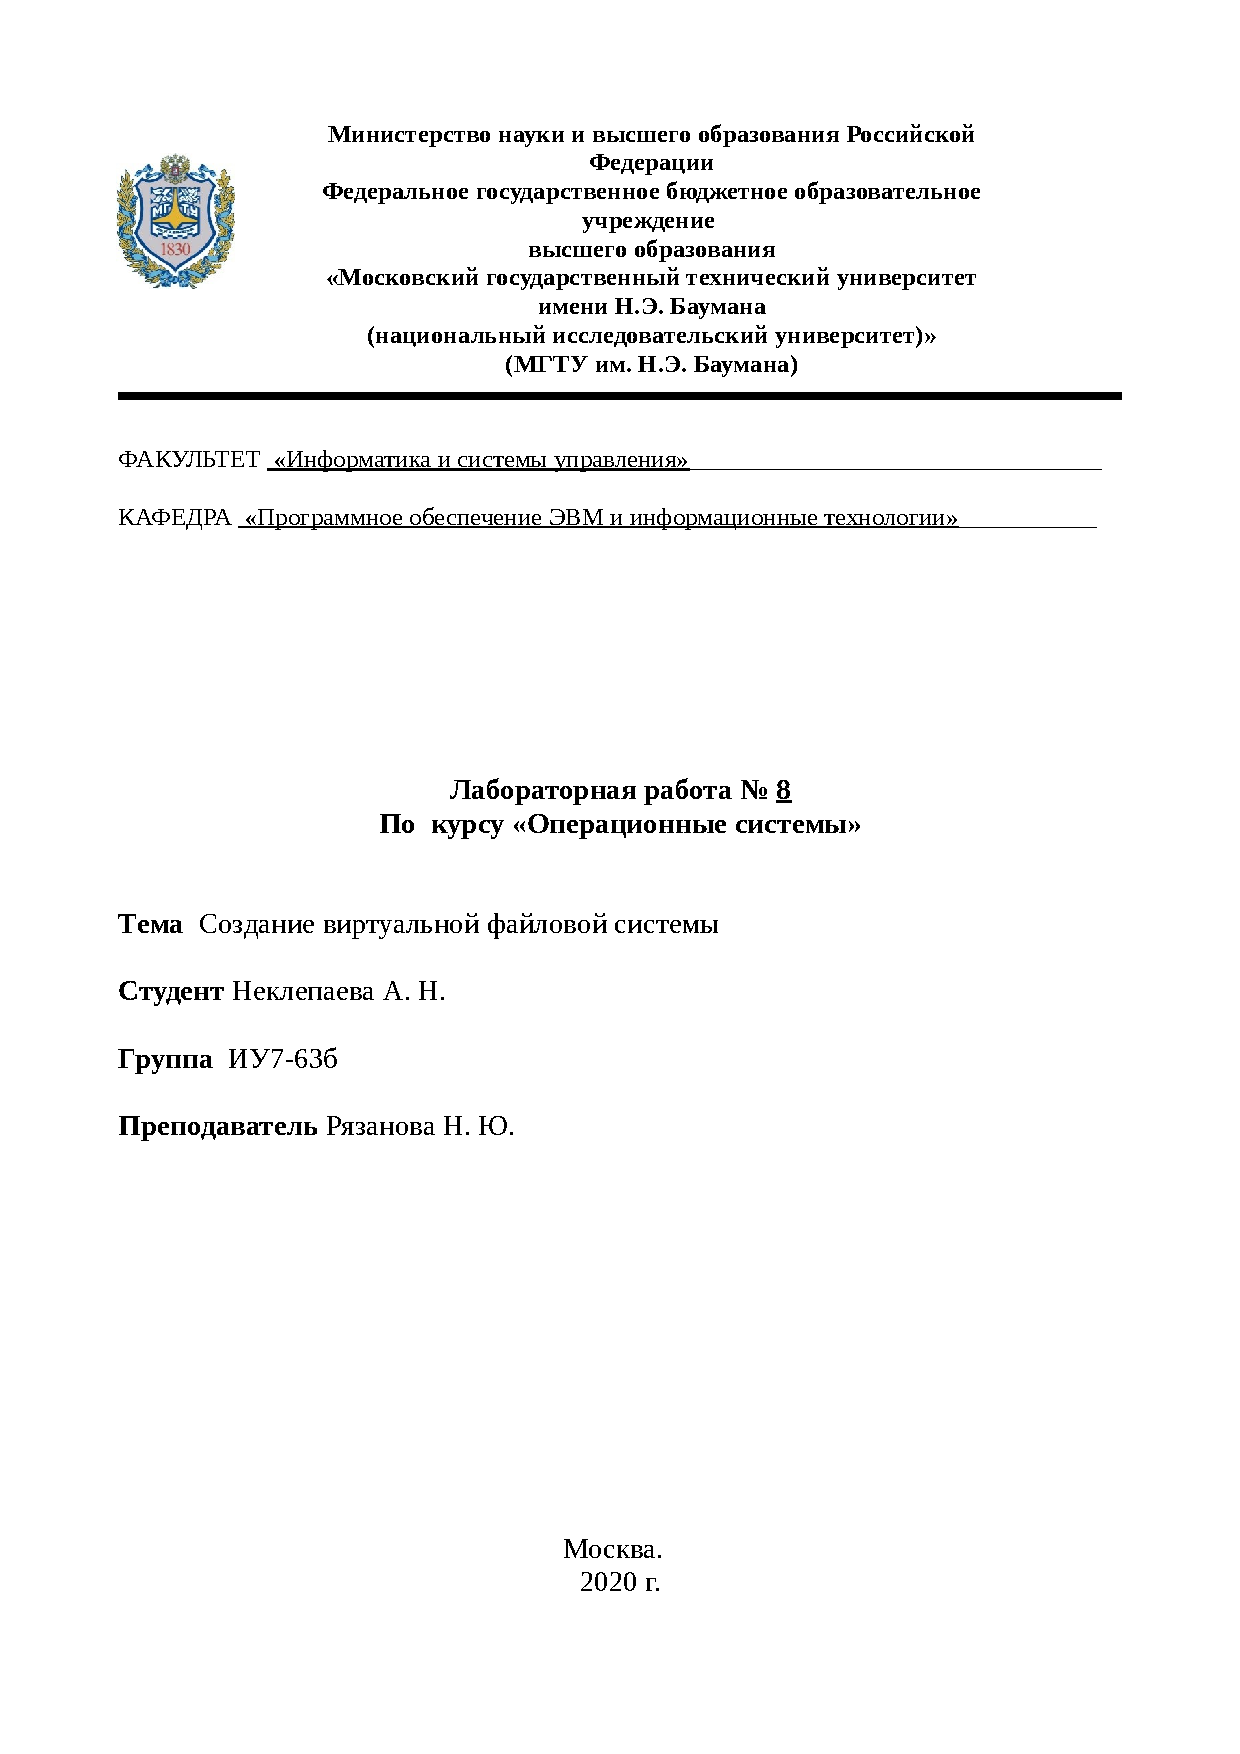
\includepdf[pages=-]{title.pdf}}
\end{figure}

\newpage

\section*{Листинг кода}

\begin{lstlisting}
  #include <linux/module.h>
  #include <linux/kernel.h>
  #include <linux/init.h>
  #include <linux/fs.h>
  #include <linux/time.h>
  #include <linux/slab.h>

  MODULE_LICENSE( "GPL" );
  MODULE_AUTHOR( "Anastasia Neklepaeva" );

  #define MAGIC_NUMBER 0x13131313

  #define SLABNAME "my_cache"
  struct kmem_cache *cache = NULL; 
  static int number = 7;
  module_param(number, int, 0); 

  struct myfs_inode
  {
      int i_mode;
      unsigned long i_ino;
  };

  static int size = sizeof(struct myfs_inode);

  // деструктор суперблока
  static void myfs_put_super(struct super_block * sb)
  {
      printk(KERN_DEBUG "MYFS super block destroyed!\n" ) ;
  }

  // put_super хранит деструктор суперблока
  static struct super_operations const myfs_super_ops = 
  {
      .put_super = myfs_put_super,
      .statfs = simple_statfs,
      .drop_inode = generic_delete_inode,

  };

  // размещение новой структуры inode 
  // и заполнение ее значениями: размером и временами
  static struct inode *myfs_make_inode(struct super_block * sb, int mode)
  {
      struct inode *ret = new_inode(sb);
      struct myfs_inode *my_inode;

      if (ret)
      {
          inode_init_owner(ret, NULL, mode);
          ret->i_size = PAGE_SIZE;
          ret->i_atime = ret->i_mtime = ret->i_ctime = current_time(ret);

          my_inode = kmem_cache_alloc(cache, GFP_KERNEL);

          my_inode->i_mode = ret->i_mode;
          my_inode->i_ino = ret->i_ino;

          ret->i_private = my_inode;
      }
      return ret;
  }

  // инициализация суперблока, построение корневого каталога
  static int myfs_fill_sb(struct super_block* sb, void* data, int silent)
  {
      struct inode* root = NULL;
      sb->s_blocksize = PAGE_SIZE;
      sb->s_blocksize_bits = PAGE_SHIFT;
      sb->s_magic = MAGIC_NUMBER;
      sb->s_op = &myfs_super_ops;

      // создание inode для корневого каталога
      root =  myfs_make_inode(sb, S_IFDIR | 0755);
      if (!root)
      {
          printk (KERN_ERR "MYFS inode allocation failed !\n") ; 
          return -ENOMEM;
      }

      root->i_op  =  &simple_dir_inode_operations;
      root->i_fop = &simple_dir_operations;
      sb->s_root  = d_make_root(root) ;

      if (!sb->s_root)
      {
          printk(KERN_ERR " MYFS root creation failed !\n") ; 
          iput(root);
          return -ENOMEM;
      }

      return 0;
  }

  // функция возвращает структуру, описывающую корневой каталог файловой системы
  static struct dentry* myfs_mount (struct file_system_type *type, int flags, 
                                      char const *dev, void *data)
  {
      struct dentry* const entry = mount_nodev(type,  flags,  data, myfs_fill_sb) ;
      if (IS_ERR(entry))
          printk(KERN_ERR  "MYFS mounting failed !\n") ;
      else
          printk(KERN_DEBUG "MYFS mounted!\n") ;
      return entry;

  }

  // структура, "описывающая" создаваемую файловую систему
  // owner отвечает за счетчик ссылок на модуль
  // name хранит название файловой системы
  static struct file_system_type myfs_type  =  
  {
      .owner  =  THIS_MODULE,
      .name  =  "myfs",
      .mount  =  myfs_mount,
      .kill_sb  =  kill_anon_super,
  };

  static int __init myfs_init(void)
  {
      // регистрация файловой системы
      int ret = register_filesystem(& myfs_type);
      if(ret != 0)
      {
          printk(KERN_ERR "MYFS_MODULE cannot register filesystem!\n");
          return ret;

      }
   
      cache = kmem_cache_create(SLABNAME, size, 0, SLAB_HWCACHE_ALIGN, NULL); 

      if (!cache)
      {
          printk( KERN_ERR "kmem_cache_create error\n"); 
          kmem_cache_destroy(cache); 
	  return -ENOMEM;
      }

      printk(KERN_DEBUG "MYFS_MODULE loaded !\n"); 
      return 0;
  }


  static void __exit myfs_exit(void)
  {
      int ret;

      // дерегистрация файловой системы
      ret = unregister_filesystem(&myfs_type); 
      if (ret != 0)
          printk(KERN_ERR "MYFS_MODULE cannot unregister filesystem !\n");
      printk(KERN_DEBUG "MYFS_MODULE unloaded !\n");

      kmem_cache_destroy(cache);
  }

  module_init( myfs_init );
  module_exit( myfs_exit );
\end{lstlisting}

\textbf{Демонстрация работы}

Загрузка модуля ядра

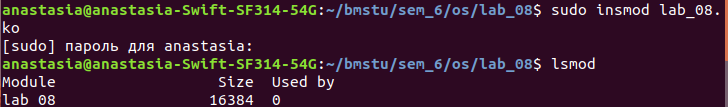
\includegraphics[scale=0.9]{1.png}

Создание образа диска и каталога, который является точкой монтирования файловой системы

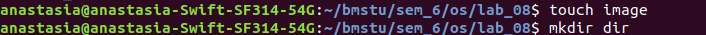
\includegraphics[scale=0.9]{2.png}

Монтирование виртуальной файловой системы, проверка системного  лога

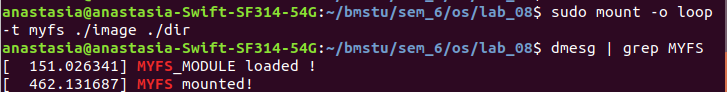
\includegraphics[scale=0.9]{3.png}

Вывод информации о виртуальной файловой системе

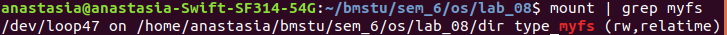
\includegraphics[scale=0.9]{4.png}

Размонтирование виртуальной файловой системы, выгрузка модуля, проверка системного лога

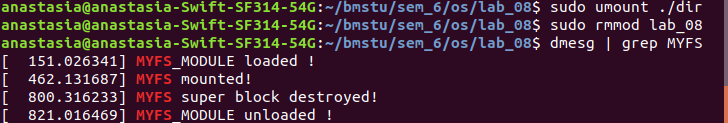
\includegraphics[scale=0.9]{5.png}

\end{document}
